\chapter{Preliminares}\label{cap:preliminares}


\section{Redes neuronales convolucionales} \label{sec:redesneuronalesconvolucionales}
Las redes neuronales convolucionales, o CNN por sus siglas en inglés, es un tipo de modelo de aprendizaje profundo para procesar datos que tiene un formato de cuadrícula, como las imágenes. Está inspirado en la organización de la corteza visual de los animales, diseñada para aprender de forma automática y adaptativa patrones en jerarquías, de bajo a alto nivel. Por lo genera una red CNN se compone de tres tipos de capas: convolución, agrupación y capas completamente conectadas, como se puede ver en la \autoref{fig:CNNEjemplo}. Las dos primeras realizan extracción de características, mientras que la tercera, las relaciona  y genera una salida. La capa de convolución desempeña un papel clave en CNN y consiste de una pila de operaciones matemáticas, como la convolución. En las imágenes en 2D estas redes son muy utilizadas, por su alta eficiencia para tareas de visión artificial, como en la clasificación y segmentación de imágenes, entre otras aplicaciones.\\

Algunos ejemplos de redes CNN son: VGG16~\cite{simonyan2014very} (que posee 13 capas de convolución, 5 de agrupación y una totalmente conectada) y AlexNet~\cite{krizhevsky2012imagenet} (que contiene 5 capas convolucionales, 3 capas de agrupación y 3 capas completamente conectadas).\\

Las redes CNN se a utilizado para resolver distintos problemas como, la detección de objetos, Fast R-CNN~\cite{girshick2015fast}, la comprensión visual de escenas de calles urbanas~\cite{cordts2016cityscapes}, entre otros. En este trabajo utilizamos la salida de las redes CNN (la capa completamente conectada), como un vector de características visual de la imagen. Debido a que las CNN son muy eficaces reconociendo patrones, si dos imágenes tienen un aspecto similar, los vectores también tendrán una semejanza.

\begin{figure}
	\centering
	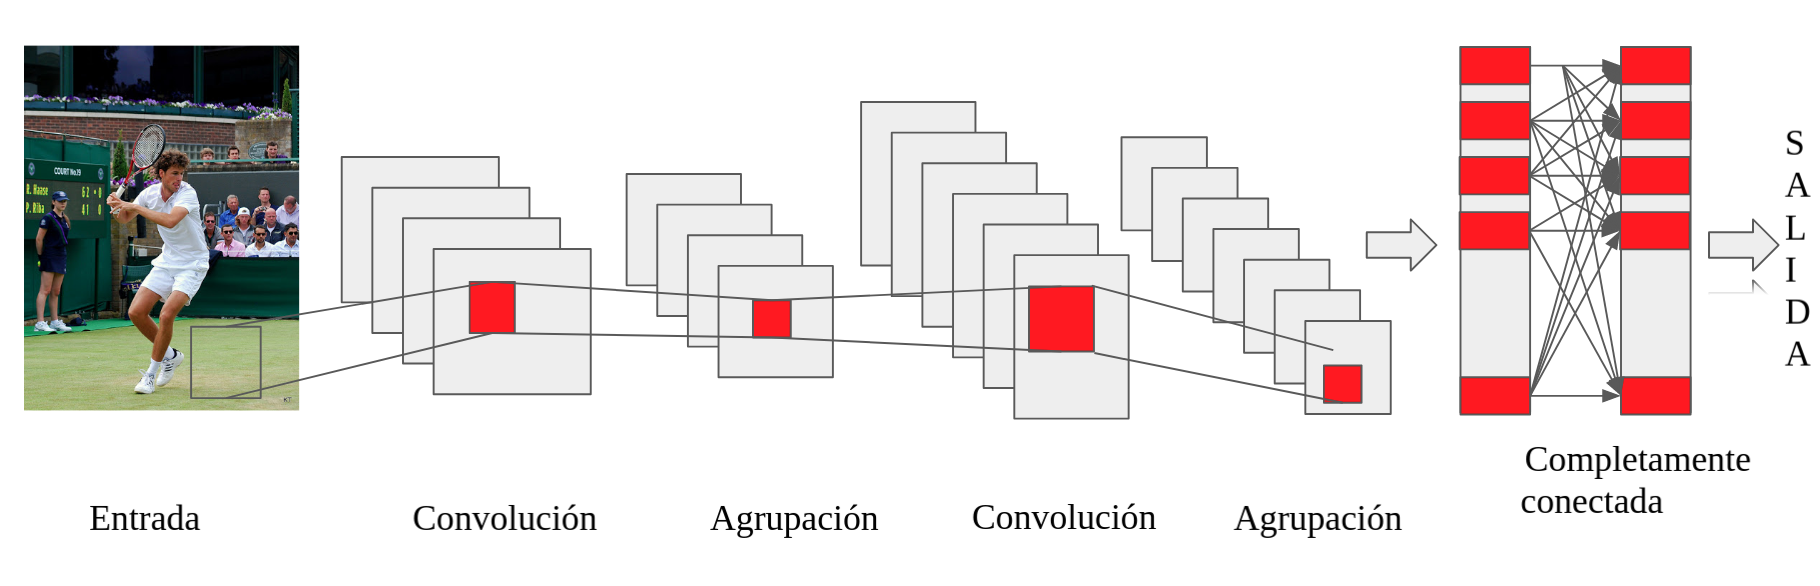
\includegraphics[width=0.9\textwidth]{img/red_cnn.png}
	\caption{Una arquitectura simplificada de una rede neuronal convolucional.}
	\label{fig:CNNEjemplo}
\end{figure}

\section{Vectores densos de palabras} \label{sec:vectoresdensosdepalabras}
Así como en las imágenes utilizamos las redes CNN, para obtener un vector que represente a la misma, es necesario un procedimiento para representar palabras con algún objeto matemático. Hay muchas formas de representar palabras, la más usada son los vectores densos de palabras, conocidos en inglés como \textit{word embedding}. Esta es una técnica de aprendizaje en el campo de procesamiento del lenguaje natural (PLN), capaz de capturar el contexto de una palabra en un documento, calcular similitud semántica y sintáctica con otras palabras.\\

Para entender como funcionan, consideremos las oraciones con un significado similar: ``Que tengas un buen día.'' y ``Que tengas un gran día.''. Si construimos un vocabulario exhaustivo:
 \[ V = \{que, tengas, un, buen, gran, dia\}. \]
A partir de esto, se puede crear un vector codificado para cada una de estas palabras, en donde cada vector tenga el tamaño de $V$, cuyos componentes sean todos 0 excepto por el elemento en el índice que representa la palabra correspondiente en el vocabulario, que contiene un 1. Esta representación no resulta conveniente ya que la distancia entre \textit{gran} y \textit{buen} es la misma que entre \textit{tengas} y \textit{buen}.  El objetivo es que las palabras con un contexto similar ocupen posiciones espaciales cercanas. Para lograr esto, se introduce cierta dependencia de una palabra con las otras.\\

Word2Vec~\cite{mikolov2013distributed} desarrollado por Tomas Mikolov en 2013. Es un modelo particularmente eficiente desde el punto de vista computacional. Este modelo se encuentra disponible de dos formas: \textit{Continuous Bag-of-Words} (CBOW) o el modelo \textit{Skip-Gram}. En CBOW, las representaciones distribuidas de contexto (o palabras circundantes) se combinan para predecir la palabra en el medio. En nuestro ejemplo \textit{gran} y \textit{buen} están rodeado de un contexto similar por lo cual resultan en vectores similares. Es varias veces más rápido de entrenar que el \textit{Skip-gram}, y tiene una precisión ligeramente mejor para las palabras frecuentes. Mientras que en el modelo \textit{Skip-gram}, la representación distribuida de la palabra de entrada se usa para predecir el contexto. Se entrena con una tarea falsa que, dada una palabra, intenta predecir las palabras vecinas. En realidad, el objetivo es solo aprender los pesos de la capa oculta que corresponden a los vectores de palabras que estamos tratando de aprender. Por ejemplo, \textit{Gran} se entrena para predecir el contexto \textit{un} y  \textit{día}, al igual que \textit{buen}. Funciona bien con una pequeña cantidad de datos de entrenamiento.

En este trabajo, aprovechamos la capacidad de capturar similitudes semántica que tiene vectores densos de palabras, para relacionar las clases vistas con las clases invisibles.\\


\section{Propuesta de objetos} \label{sec:propuestadeobjetos}
En problemas de detección de objetos, generalmente se tiene que encontrar todos los objetos posibles en la imagen. La localización de objetos se refiere a identificar la ubicación de uno o varios objetos en la imagen. Un algoritmo de localización de objetos generará las coordenadas de la ubicación de los objetos con respecto a la imagen. En visión artificial, la forma más popular de representar la ubicación de los objetos es con la ayuda de cuadros delimitadores (\textit{Bounding Boxs}). Existen muchos algoritmos y redes que intenta resolver este problema, algunos ejemplos son ventana deslizante (\textit{slide window}), Edge-Boxes~\cite{zitnick2014edge} y búsqueda selectiva (\textit{selective search})~\cite{uijlings2013selective}. En ZSD la propuesta de objetos cumple un papel importante, ya que se necesita extraer todas las instancias de los objetos, pero también tiene que discriminar fondos como cielo, ciudades, veredas, etc.\\

En este proyecto, como veremos en el \autoref{cap:experimentos} se experimentó con Edge-Boxes y \textit{selective search}, ya que estas generan una cantidad de propuestas significativamente menor a algoritmos del estilo de ventana deslizante. Aun así, procesar todas estas propuestas es engorroso. Adamas, estos modelos por lo general dan como resultados muchos cuadros con una gran superposición. Esto da lugar a una técnica denominada supresión no máxima (NMS), ejemplificada en la~\autoref{fig:NMS}. Este algoritmo necesita de un puntaje que indica la confianza del cuadro delimitador y un criterio para comparar entre distintos cuadros. El criterio más común es Intersección sobre Unión (IoU), en la~\autoref{fig:IoU} se muestra como se calcula sobre dos \textit{Bounding Boxs}. La salida de NMS es un conjunto más reducido de propuestas, en la cual se filtraron todas las que se consideran repetidas y retorna solo las más representativa. A continuación se muestra el pseudocódigo de NMS.

\begin{center}
\noindent\fbox{
	\begin{minipage}{1\textwidth}
		\begin{algorithmic}[1]
			\Procedure{NMS}{B, S, t}
				\State{D = $\emptyset$ }
				\For {B $\neq \emptyset$ }
					\State{$b_i$ = \textbf{SelPropuestaMaxPuntaje}(B, S)}
					\State{\textbf{Eliminar}($b_i$, B)}
					\For {$b_j$ $\in$ B}
						\If {\textbf{IoU}($b_i$, $b_j$) $>$ t}
							\State{\textbf{Eliminar}($b_j$, B)}
						\EndIf
					\EndFor				
				\EndFor
			\State{\Return {D}}
			\EndProcedure
		\end{algorithmic}
	\end{minipage}
}
\end{center}

\begin{figure}[]
	\begin{subfigure}{.5\textwidth}
		\centering
		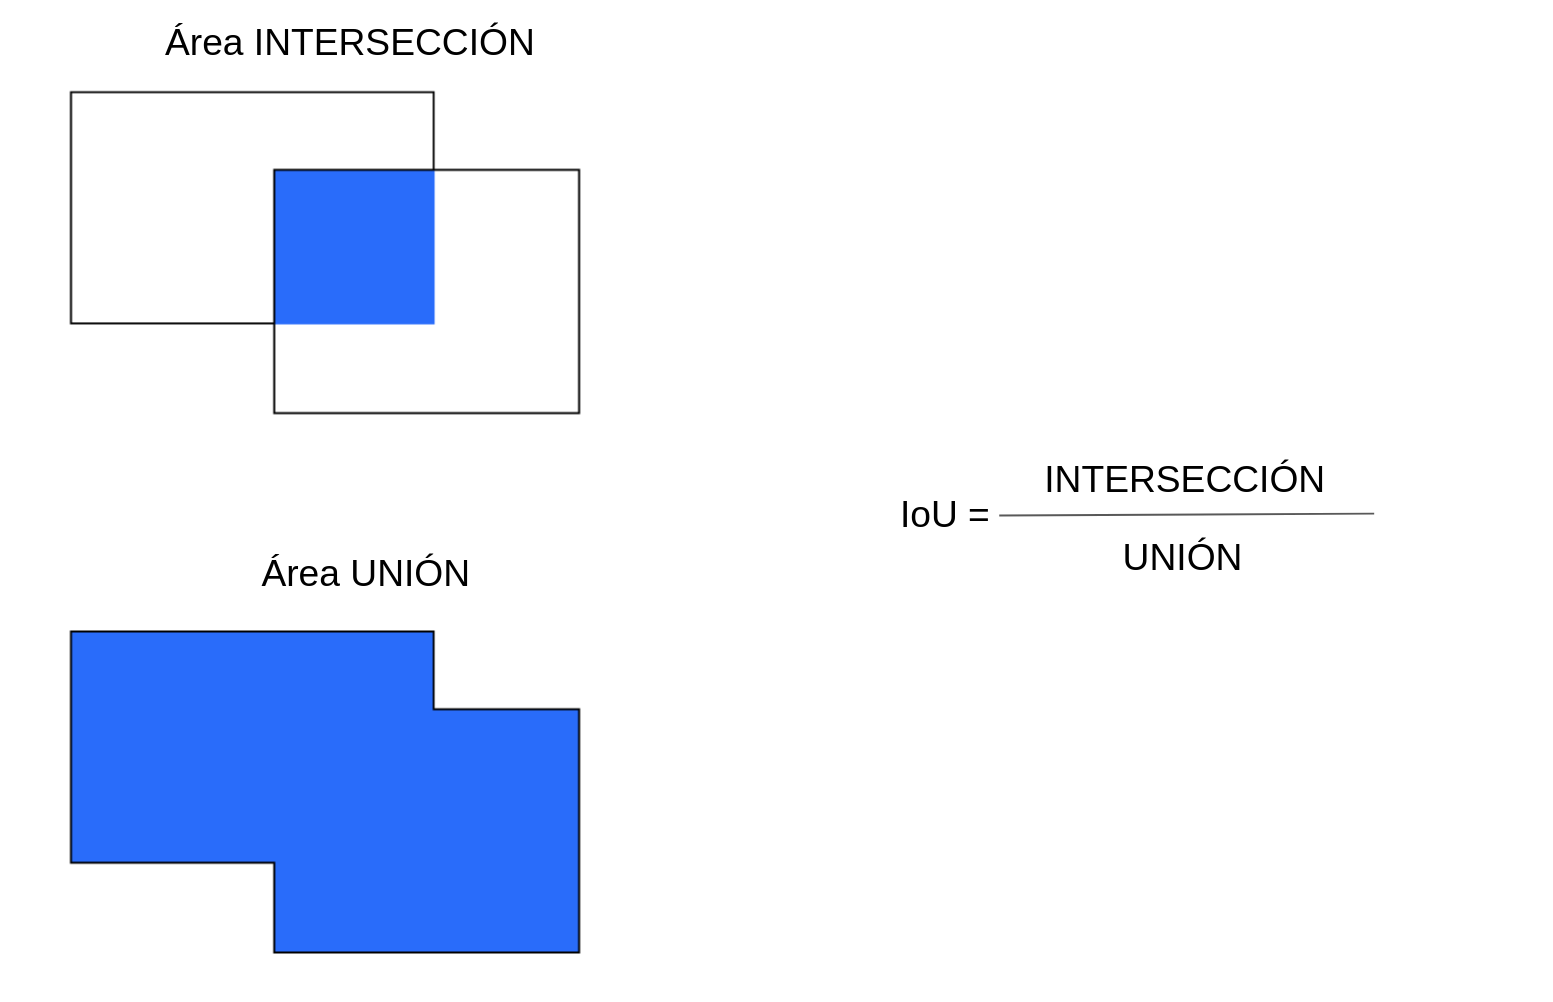
\includegraphics[width=0.7\textwidth]{img/iou.png}
		\caption{IoU}
		\label{fig:IoU}
	\end{subfigure}
	\begin{subfigure}{.5\textwidth}
		\centering
		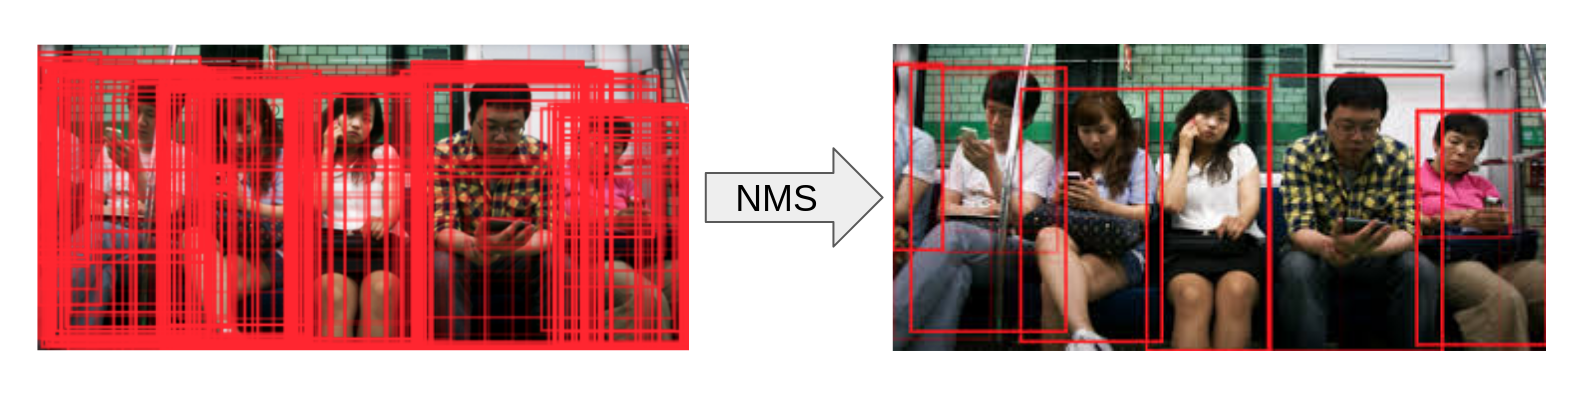
\includegraphics[width=1.1\textwidth]{img/NMS.png}
		\caption{Supresión no máxima}
		\label{fig:NMS}
	\end{subfigure}
	\caption{(a) Calculo de Intersección sobre Unión. (b) Salida de la propuesta de objetos y el resultado después de NMS.}
		\label{fig:RP}
\end{figure}

\section{Multimodales} \label{sec:multimodales}

Nuestra experiencia del mundo es multimodal, vemos objetos y sus entornos, escuchamos música y ruidos, sentimos la textura de los distintos materiales, etc.  Inconscientemente asociamos una situación a los distintos estímulos que recibimos en ese momento y los relacionamos entre si, para genera una idea de lo que esta sucediendo. De esta manera, sabemos que si algo huele mal, lo más probable es que sepa igual, o podemos relacionar una imagen del campo con el sonido de los pájaros.\\

La modalidad se refiere a la forma en que algo sucede o se experimenta. Un problema de investigación se caracteriza como multimodal cuando incluye datos de distinta naturaleza. Para que la inteligencia artificial avance en la comprensión del mundo que nos rodea, necesita poder interpretar y relacionar estas distintas señales. Si bien la combinación de diferentes modalidades para mejorar el rendimiento parece una tarea intuitivamente atractiva, en la práctica, es un desafío, ya que una ineducada combinación de distintos tipos de información, puede generar confusión y conflictos. 

La idea general es, a partir de dos objetos matemáticos distintos, uno de cada modal, poder transformarlos para lograr que pertenezcan a un tercer objeto que corresponde a la representación multimodal. Las imágenes suelen estar asociadas con etiquetas y explicaciones de texto. En este trabajo nos aprovechamos de esto y tratamos de encontrar un espacio común entre el vector que representan a la imagen del objeto y el que representa la sintaxis de la clase.

\section {Aprendizaje por disparo cero (ZSL)} \label{sec:aprendizajepordisparocero}
ZSL es un conjunto de problemas de aprendizaje automático, donde en el momento de la prueba, se observan muestras de clases que no se observaron durante el entrenamiento y se necesita predecir la categoría a la que pertenecen. Esta se diferencia de las configuraciones estándares en el aprendizaje automático, donde se espera que se clasifiquen correctamente las nuevas muestras en las clases que ya se han observado durante el entrenamiento.
Podemos diferenciar dos tipos de clases, las vistas que están presente en el entrenamiento y las invisibles o novedosas que no estuvieron en el mismo. Se debe proporcionar algún tipo de información complementaria sobre estas clases invisibles, este tipo de dato puede ser variado. Como por ejemplo, una descripción estructurada predefinida, que al tenerla en cuenta mejora el aprendizaje, o una descripción textual, donde las clases van acompañadas de un comentario en lenguaje natural, etc. Por último, tanto las clases visibles como las invisibles están relacionadas en un espacio vectorial, donde el conocimiento de las clases vistas se puede transferir a clases invisibles.\\

El problema de aprendizaje por disparo cero se puede dividir en categorías según los datos presentes durante la fase de entrenamiento y la fase de prueba:
\begin{itemize}
	\item En base a los datos disponibles en el momento de entrenar un modelo.
	\begin{itemize}
		\item \textbf{Aprendizaje por disparo cero inductivo:} Se tiene acceso a los datos y a la información complementario de solo las clases vistas.
		\item \textbf{Aprendizaje por disparo cero transductivo:} Además de los datos y la información complementario de las clases vistas,  se tiene acceso a los datos de las clases no vistas.
	\end{itemize}
	\item Basado en los datos disponibles en el momento de la inferencia.
	\begin{itemize}
		\item \textbf{Aprendizaje por disparo cero convencional (ZSL):} En las pruebas solo se evalúan las clases no vistas.
		\item \textbf{Aprendizaje por disparo cero generalizado (GZSL):} En las pruebas se evalúan tanto las clases vista como las no vistas.
	\end{itemize}
\end{itemize}

\section {Detección de objeto por disparo cero (ZSD)} \label{sec:detecciondeobjetopordisparocero}
La Detección de objeto por disparo cero (ZSD), tiene como objetivo reconocer y localizar simultáneamente instancias de objetos que pertenecen a categorías novedosas sin ningún ejemplo de entrenamiento. Como estas categorías no están presente en el entrenamiento, no se tiene ninguna información sobre su aspecto visual, lo cual no nos permite detectarlas ni reconocerlas. Por lo tanto, es necesario encontrar algún dominio que tenga la capacidad de guardar la información de todas las clases, para luego relacionarlas con el aspecto visual de las categorías novedosas.

Este trabajo se basa en el artículo científico de Bansal \etal ~\cite{bansal2018zero}, además utiliza muchos conceptos sobre disparo cero generalizado~\cite{zero-shot-generalizado}. Se propone un modelo de disparo cero inductivo, es decir, solo se observan imágenes de clases vistas y etiquetas que indican a que clase pertenece. Estas etiquetas son palabras del lenguaje natural sin ninguna estructura. Luego, se puede inferir todas las clases o solo las invisibles, dependiendo de si se quiere evaluar aprendizaje por disparo cero generalizado o convencional, respectivamente.\\ 

El requisito estricto de no utilizar ninguna imagen de clase invisible durante el entrenamiento es una condición difícil. Además, existen otras dificultades en la tarea de detección de disparo cero relacionadas al conjunto de datos de entrenamiento y prueba, es decir entre las clases vistas e invisibles. Estas dificultades son:

\begin{itemize}
	\item \textbf{Rareza}: los conjuntos de datos, por lo general, contiene un problema de distribución, es decir, muchas clases raras tienen menos cantidad de instancias. Este problema hace que las clases con mayor cantidad de instancias sesguen el modelo y las clases más raras sean marcadas incorrectamente en la etapa de prueba. Esto es un problema al momento de comparar dos modelos que fueron entrenados con distintas clases, ya que algunas separaciones  de las clases resultan mejores que otras.

	\item \textbf{Tamaño del objeto}: algunas clases de objetos raros (tijeras, lápices, celulares, etc.), suelen tener un tamaño pequeño. Los objetos más pequeños son difíciles de detectar y reconocer. También, tienen el problema de que por lo general están junto a objetos más grandes como una mesa o una persona y se ven opacadas por estas clases.

	\item \textbf{Diversidad}: cuando una clase invisible no tiene otras clases visualmente similares, resulta muy difícil aprender el aspecto visual de esta. Por ejemplo, ``auto'' tiene muchas clases similares en comparación con ``cartel''. Esto permite una descripción visual inadecuada de la clase invisible ``cartel'' que eventualmente afectará el rendimiento de detección de disparo cero, a diferencia de lo que sucede con la clase ``auto''.

	\item \textbf{Ruido en el espacio semántico}: cuando se utiliza los vectores de incrustación semántica no supervisados como Word2Vec~\cite{mikolov2013distributed} o GloVe~\cite{pennington2014glove}, las incrustaciones resultante en general son ruidosas, ya que se generan automáticamente a partir de la minería de texto no anotado. Esto también afecta significativamente el rendimiento de la detección de disparo cero.
\end{itemize}

Existen algunas variaciones de ZSD que intentan atenuar estos problemas, agrupando las clases en grupos o metaclases. Estas variaciones son: 

\begin{itemize}

	\item \textbf{Detección de metaclase de disparo cero (ZSMD)}, que dada una imagen de prueba, el objetivo es localizar cada instancia de una clase de objeto invisible y categorizarla en una de las superclases.

	\item \textbf{Etiquetado de disparo cero (ZST)}, consiste en reconocer una o más clases invisibles en una imagen de prueba, sin identificar su ubicación.

	\item \textbf{Etiquetado de metaclase de disparo cero (ZSMT)}, reconoce una o más metaclases en una imagen de prueba, sin identificar su ubicación.

\end{itemize}

	Estas tareas son atractivas a la hora de calcular métricas, pero no para ser aplicadas a problemas reales.